\chapter{Categorical organisation of the ornament--refinement framework}
\label{chap:categorical}

\begin{figure}
\begin{center}
\begin{tikzpicture}[x=4em, y=4em, baseline=(Fun.base)]
\node(Orn) {|Ōrn|};
\node(Fam) [below=1.5 of Orn] {|Fam|};
\node(FRef) [left=1 of Fam] {|FRef|};
\node(Fun) [right=2.5 of Fam] {|Fun|};
\path[->]
(Orn)             edge[bend right]              node[above left] {|RSem|}  (FRef)
(Orn)             edge                          node[right]      {|Ind|}   (Fam)
(FRef.north east) edge[bend left]               node[above]      {|FRefF|} (Fam.north west)
(Fam.south west)  edge[bend left]               node[below]      {|FRefC|} (FRef.south east)
(Fam)             edge[bend left,looseness=.7]  node[above]      {|Com|}   (Fun)
(Fam)             edge[bend right,looseness=.7] node[below]      {|FamF|}  (Fun);
\node at ($(FRef)!.5!(Fam)$) {|≅*|};
\end{tikzpicture}
\end{center}
\caption{Categories and functors for the ornament--refinement framework.}
\label{fig:categories}
\end{figure}

\autoref{chap:refinements-and-ornaments} left some obvious holes in the theory of ornaments.
For instance:
\begin{itemize}
\item When it comes to composition of ornaments, the following \key{sequential composition} is probably the first that comes to mind (rather than parallel composition), which is evidence that the ornamental relation is transitive:
\begin{code}
_⊙_ :  {I J K : Set} {e : J → I} {f : K → J} →
       {D : Desc I} {E : Desc J} {F : Desc K} →
       Orn e D E → Orn f E F → Orn (e ∘ f) D F
-- definition in \autoref{fig:sequential-composition}
\end{code}
Correspondingly, we expect that
\[ |forget (O ⊙ P)| \qquad\text{and}\qquad |forget O ∘ forget P| \]
are extensionally equal.
That is, the sequential compositional structure of ornaments corresponds to the compositional structure of forgetful functions.
We wish to state such correspondences in concise terms.
\item While parallel composition of ornaments~(\autoref{sec:parallel-composition}) has a sensible definition, it is defined by case analysis at the \emph{microscopic} level of individual fields.
Such a microscopic definition is difficult to comprehend, and so are any subsequent definitions and proofs.
It is desirable to have a \emph{macroscopic} characterisation of parallel composition, so the nature of parallel composition is immediately clear, and subsequent definitions and proofs can be done in a more abstract manner.
\item The ornamental conversion isomorphisms~(\autoref{sec:optimised-predicates}) and the modularity isomorphisms~(\autoref{sec:predicate-swapping}) were left unimplemented.
Both sets of isomorphisms are about the optimised predicates~(\autoref{sec:optimised-predicates}), which are defined in terms of parallel composition with singleton ornamentation~(\autoref{sec:ornamental-descriptions}).
We thus expect that the existence of these isomorphisms can be explained in terms of properties of parallel composition and singleton ornamentation.
\end{itemize}
A lightweight organisation of the ornament--refinement framework in basic category theory~\citep{MacLane-categories} can help to fill in all these holes.
In more detail:
\begin{itemize}
\item Categories and functors are abstractions for compositional structures and structure-preserving maps between them.
Facts about translations between ornaments, refinements, and functions can thus be neatly organised under the categorical language (\autoref{sec:categories-and-functors}).
The categories and functors used in this chapter are summarised in \autoref{fig:categories}.
\item Parallel composition merges two compatible ornaments and does nothing more; in other words, it computes the least informative ornament that contains the information of both ornaments.
Characterisation of such \key{universal constructions} is a speciality of category theory; in our case, parallel composition can be shown to be a categorical \key{pullback}~(\autoref{sec:parallel-composition-pullback}).
\item Universal constructions are unique up to isomorphism, so it is convenient for establishing isomorphisms about universal constructions.
The status of parallel composition being a pullback can thus help to construct the ornamental conversion isomorphisms (in \autoref{sec:ornamental-conversion-isomorphisms}) and the modularity isomorphisms (in \autoref{sec:modularity-isomorphisms}).
\end{itemize}
\autoref{sec:categorical-discussion} concludes with some discussion.

\section{Categories and functors}
\label{sec:categories-and-functors}

We define the general notions of categories and functors in \autoref{sec:basic-categorical-definitions} and then concrete categories and functors specifically about ornaments and refinements in \autoref{sec:concrete-categories}.
Categories and functors by themselves are uninteresting, though; it is the purely categorical structures defined on top of categories and functors that make the categorical language worthwhile.
We introduce the first such definition --- categorical isomorphisms --- in \autoref{sec:isomorphisms}, and more in \autoref{sec:parallel-composition-pullback}.

\subsection{Basic definitions}
\label{sec:basic-categorical-definitions}

A first approximation of a category is a (directed multi-) \key{graph}, which consists of a set of objects (nodes) and a collection of sets of morphisms (edges) indexed with their source and target objects:
\begin{code}
record ^^^Graph {l m : Level} : Set (suc (l ⊔ m)) where
  field
    Object    :  Set l
    _==>_     :  Object → Object → Set m
\end{code}
For example, the underlying graph of the category |Fun| of (small) sets and (total) functions is
\begin{code}
^^^Fun-graph : Graph
Fun-graph = record  case  Object  = Set
                    sep   _==>_   = (lambda(A B)) A → B endcase
\end{code}
A category is a graph whose morphisms are equipped with a monoid-like compositional structure --- there is a morphism composition operator of type
\begin{code}
_·_  : {X Y Z : Object} → (Y ==> Z) → (X ==> Y) → (X ==> Z)
\end{code}
which has left and right identities and is associative.

\block{Remark}{universe polymorphism}{Many definitions in this chapter (like |Graph| above) employ \Agda's \key{universe polymorphism}~\citep{Harper-universes}, so the definitions can be instantiated at suitable levels of the |Set| hierarchy as needed.
(For example, the type of |Fun-graph| is implicitly instantiated as |Graph {1} {0}|, since |Set| is of type |Set₁| and any |A → B| (where |A|, |B : Set|) are of type |Set| ($=$~|Set₀|), and |Graph {1} {0}| itself is of type |Set₂|, whose level is computed by taking the successor of the maximum of the two level arguments.)
We will give the first few universe-polymorphic definitions with full detail about their levels, but will later suppress the syntactic noise wherever possible.}

Before we move on to the definition of categories, though, special attention must be paid to equality on morphisms, which is usually coarser than definitional equality --- in |Fun|, for example, it is necessary to identify functions up to extensional equality (so uniqueness of morphisms in universal properties would make sense).
As stated in \autoref{sec:equality}, such equalities need to be explicitly managed in \Agda's intensional setting, and one way is to use \key{setoids}~\citep{Barthe-setoids} --- sets with an explicitly specified equivalence relation --- to represent sets of morphisms.
Subsequently, functions defined between setoids need to be proved to respect the equivalences.
The type of setoids can be defined as a record which contains a carrier set, an equivalence relation on the set, and the three laws for the equivalence relation:
\begin{code}
record ^^^Setoid {c d : Level} : Set (suc (c ⊔ d)) where
  field
    Carrier  : Set c
    _≈_      : Carrier → Carrier → Set d

    refl'  : {x : Carrier} → x ≈ x
    sym    : {x y : Carrier} → x ≈ y → y ≈ x
    trans  : {x y z : Carrier} → x ≈ y → y ≈ z → x ≈ z
\end{code}
For example, we can define a setoid of functions that uses extensional equality:
\begin{code}
^^^FunSetoid : Set → Set → Setoid
FunSetoid A B = record  case  Carrier  =  A → B
                        sep   _≈_      =  _≐_
                        sep   proofs-of-laws endcase
\end{code}
Proofs of the three laws are omitted from the presentation.

\begin{figure}
\codefigure\small
\begin{code}
record ^^^Category {l m n : Level} : Set (suc (l ⊔ m ⊔ n)) where
  field
    Object    :  Set l
    Morphism  :  Object → Object → Setoid {m} {n}

  _==>_ : Object → Object → Set m
  X ==> Y = Setoid.Carrier (Morphism X Y)
  _≈_ : {X Y : Object} → (X ==> Y) → (X ==> Y) → Set n
  _≈_ {X} {Y} = Setoid._≈_ (Morphism X Y)

  field
    _·_  :   {X Y Z : Object} → (Y ==> Z) → (X ==> Y) → (X ==> Z)
    id   :   {X : Object} → (X ==> X)

    id-l    :  {X Y : Object} (f : X ==> Y) → id · f ≈ f
    id-r    :  {X Y : Object} (f : X ==> Y) → f · id ≈ f
    assoc   :  {X Y Z W : Object} (f : Z ==> W) (g : Y ==> Z) (h : X ==> Y) →
               (f · g) · h ≈ f · (g · h)
    cong-l  :  {X Y Z : Object} {f g : Y ==> Z} (h : X ==> Y) → f ≈ g → f · h ≈ g · h
    cong-r  :  {X Y Z : Object} (h : Y ==> Z) {f g : X ==> Y} → f ≈ g → h · f ≈ h · g

record ^^^Functor {l m n l' m' n' : Level}
  (C : Category {l} {m} {n}) (D : Category {l'} {m'} {n'}) :
  Set (l ⊔ m ⊔ n ⊔ l' ⊔ m' ⊔ n') where
  field
    object    :  Object C → Object D
    morphism  :  {X Y : Object C} → X =C=> Y → object X =D=> object Y

    equiv-preserving  :  {X Y : Object C} {f g : X =C=> Y} →
                         f ≈C g → morphism f ≈D morphism g
    id-preserving     :  {X : Object C} → morphism (id C {X}) ≈D id D {object X}
    comp-preserving   :  {X Y Z : Object C} (f : Y =C=> Z) (g : X =C=> Y) →
                         morphism (f ·C g) ≈D (morphism f ·D morphism g)
\end{code}
\caption{Definitions of categories and functors. Subscripts are used to indicate to which category an operator belongs.}
\label{fig:definitions-of-categories-and-functors}
\end{figure}

The type of categories is then defined as a record containing a set of objects, a collection of \emph{setoids} of morphisms indexed by source and target objects, the composition operator on morphisms, the identity morphisms, and the identity and associativity laws for composition.
The definition is shown in \autoref{fig:definitions-of-categories-and-functors}.
Two notations are introduced to improve readability: |X ==> Y| is defined to be the carrier set of the setoid of morphisms from~|X| to~|Y|, and |f ≈ g| is defined to be the equivalence between the morphisms |f|~and~|g| as specified by the setoid to which |f|~and~|g| belong.
The last two laws |cong-l| and |cong-r| require morphism composition to preserve the equivalence on morphisms; they are given in this form to work better with the equational reasoning combinators commonly used in \Agda\ (see, e.g., the \name{AoPA} library~\citep{Mu-AoPA}).

\begin{figure}
\codefigure\small\vskip-1\baselineskip
\begin{code}
^^^Fam : Category
Fam = record
  case  Object    =  (Σ'(I ∶ Set)) I → Set
  sep   Morphism  =  λ case  (J , Y) (I , X) mapsto record
                               case  Carrier  = (Σ'(e ∶ J → I)) Y ⇉ (X ∘ e)
                               sep   _≈_      = λ case  (e , u) (e' , u') mapsto
                                                          (e ≐ e') × ((j : J) → u {j} ≊' u' {j}) endcase
                               sep  proofs-of-laws endcase endcase
  sep   _·_  = λ case (e , u) (f , v) mapsto e ∘ f , ((lambda({k})) u {f k} ∘ v {k}) endcase
  sep   id   =  ((lambda(x)) x) , ((lambda({i} x)) x)
  sep   proofs-of-laws endcase

^^^FRef : Category
FRef = record
  case  Object    =  (Σ'(I ∶ Set)) I → Set
  sep   Morphism  =  λ case  (J , Y) (I , X) mapsto record
                               case  Carrier  = (Σ'(e ∶ J → I)) FRefinement e X Y
                               sep   _≈_      = λ case  (e , rs) (e' , rs') mapsto
                                                          (e ≐ e') ×
                                                          ((j : J) →  Refinement.forget (rs   (ok j)) ≊'
                                                                      Refinement.forget (rs'  (ok j))) endcase
                               sep  proofs-of-laws endcase endcase
  sep   proofs-of-laws endcase

^^^Ōrn ^^^Orn' : Category
Ōrn = record
  case  Object    =  (Σ'(I ∶ Set)) Desc I
  sep   Morphism  =  λ case  (J , E) (I , D) mapsto record
                               case  Carrier  = (Σ'(e ∶ J → I)) Orn e D E
                               sep   _≈_      = λ case (e , O) (f , P) mapsto OrnEq O P endcase
                               sep  proofs-of-laws endcase endcase
  sep   _·_  =  λ case (e , O) (f , P) mapsto e ∘ f , O ⊙ P endcase
  sep   id   =  λ case {I , D} mapsto ((lambda(i)) i) , idOrn D endcase
  sep   proofs-of-laws endcase
\end{code}
\caption{(Partial) definitions of the categories |Fam|, |FRef|, and |Ōrn|.}
\label{fig:concrete-categories}
\end{figure}

Now we can define the category |Fun| of sets and functions as
\begin{code}
^^^Fun : Category
Fun = record  case  Object    =  Set
              sep   Morphism  =  FunSetoid
              sep   _·_  =  _∘_
              sep   id   =  (lambda(x)) x
              sep   proofs-of-laws endcase
\end{code}
Another important category that we will make use of is |Fam|~(\autoref{fig:concrete-categories}), the category of indexed families of sets and indexed families of functions, which is useful for talking about componentwise structures.
An object in |Fam| has type |(Σ'(I ∶ Set)) I → Set|, i.e., it is a set~|I| and a family of sets indexed by~|I| \sidenote{forming this |Σ|-type requires a universe-polymorphic revision of the definition of~|Σ|};
a morphism from |(J , Y)| to |(I , X)| is a function |e : J → I| and a family of functions from |Y j| to |X (e j)| for each |j : J|.
Morphism composition is componentwise composition, and morphism equivalence is defined to be componentwise extensional equality.
(The morphism equivalence is formulated with the help of McBride's ``John Major'' heterogeneous equality~|^^^_≊_|~\citep{McBride-thesis} --- the equivalence~|^^^_≊'_| is pointwise heterogeneous equality --- since given |y : Y j| for some |j : J|, the types of |u {j} y| and |u' {j} y| are not definitionally equal but only provably equal.)

Categories are graphs with a compositional structure, and \key{functors} are transformations between categories that preserve the compositional structure.
The definition of functors is shown in \autoref{fig:definitions-of-categories-and-functors}: a functor consists of two mappings, one on objects and the other on morphisms, where the morphism part preserves all structures on morphisms, including equivalence, identity, and composition.
For example, we have two functors from |Fam| to |Fun|, one summing components together
\begin{code}
^^^Com : Functor Fam Fun  -- the comprehension functor
Com = record  case  object    =  λ case (I  ,  X  ) mapsto Σ I X  endcase
              sep   morphism  =  λ case (e  ,  u  ) mapsto e * u  endcase
              sep   proofs-of-laws endcase
\end{code}
and the other extracting the index part.
\begin{code}
^^^FamF : Functor Fam Fun  -- the family fibration functor
FamF = record  case  object    =  λ case (I  ,  X  ) mapsto I  endcase
               sep   morphism  =  λ case (e  ,  u  ) mapsto e  endcase
               sep   proofs-of-laws endcase
\end{code}
Proofs of the functor laws are omitted from the presentation.

\subsection{Categories and functors for refinements and ornaments}
\label{sec:concrete-categories}

Some constructions in \autoref{chap:refinements-and-ornaments} can now be organised under several categories (whose definitions are shown in \autoref{fig:concrete-categories}) and functors.
For a start, we already saw that refinements are interesting only because of their intensional contents; extensionally they amount only to their forgetful functions.
This is reflected in an \emph{isomorphism} of categories between the category |Fam| and the category |FRef| of type families and refinement families (i.e., there are two functors back and forth inverse to each other).
An object in |FRef| is an indexed family of sets as in |Fam|, and a morphism from |(J , Y)| to |(I , X)| consists of a function |e : J → I| on the indices and a refinement family of type |FRefinement e X Y|.
As for the equivalence on morphisms, it suffices to use extensional equality on the index functions and componentwise extensional equality on refinement families, where extensional equality on refinements means extensional equality on their forgetful functions (extracted by |Refinement.forget|), which we have shown in \autoref{sec:individual-refinements} to be the core of refinements.
Note that a refinement family from |X : I → Set| to |Y : J → Set| is deliberately cast as a morphism in the opposite direction from |(J , Y)| to |(I , X)|; think of this as suggesting the direction of the forgetful functions of refinements.
We can then define the following two functors, forming an isomorphism of categories between |FRef| and |Fam|:
\begin{itemize}
\item We have a forgetful functor |FRefF : Functor FRef Fam| which is identity on objects and componentwise |Refinement.forget| on morphisms (which preserves equivalence automatically):
\begin{code}
^^^FRefF : Functor FRef Fam
FRefF = record
  case  object     = id
  sep   morphism   = λ case (e , rs) mapsto e , ((lambda(j)) Refinement.forget (rs (ok j))) endcase
  sep   proofs-of-laws endcase
\end{code}
Note that |FRefF| remains a familiar covariant functor rather than a contravariant one because of our choice of morphism direction.
\item Conversely, there is a functor |FRefC : Functor Fam FRef| whose object part is identity and whose morphism part is componentwise |canonRef|:
\begin{code}
^^^FRefC : Functor Fam FRef
FRefC = record
  {    object    =  id
  sep  morphism  =  λ case (e , u) mapsto e , λ case (ok j) mapsto canonRef (u {j}) endcase endcase
  sep  proofs-of-laws }
\end{code}
\end{itemize}
The two functors |FRefF| and |FRefC| are inverse to each other by definition.

\begin{figure}
\codefigure\small
\begin{code}
^^^Ė-refl ^^^E-refl : (is : List I) → Ė id is is
Ė-refl []        = []
Ė-refl (i ∷ is)  = refl ∷ Ė-refl is

^^^idROrn : (E : RDesc I) → ROrn id E E
idROrn (ṿ is)   = ṿ (Ė-refl is)
idROrn (σ S E)  = (σ'(s ∶ S)) idROrn (E s)

^^^idOrn : {I : Set} (D : Desc I) → Orn id D D
idOrn {I} D (ok i) = idROrn (D i)

^^^Ė-trans ^^^E-trans :  {I J K : Set} {e : J → I} {f : K → J} →
              {is : List I} {js : List J} {ks : List K} →
              Ė e js is → Ė f ks js → Ė (e ∘ f) ks is
Ė-trans           []            []            =  []
Ė-trans {e := e}  (eeq ∷ eeqs)  (feq ∷ feqs)  =  trans (cong e feq) eeq ∷ Ė-trans eeqs feqs

^^^scROrn :  {I J K : Set} {e : J → I} {f : K → J} →
             {D : RDesc I} {E : RDesc J} {F : RDesc K} →
             ROrn e D E → ROrn f E F → ROrn (e ∘ f) D F
scROrn (ṿ eeqs)  (ṿ feqs)  = ṿ (Ė-trans eeqs feqs)
scROrn (ṿ eeqs)  (Δ T P)   = (Δ'(t ∶ T))  scROrn (ṿ eeqs)  (P t)
scROrn (σ S O)   (σ .S P)  = (σ'(s ∶ S))  scROrn (O s)     (P s)
scROrn (σ S O)   (Δ T P)   = (Δ'(t ∶ T))  scROrn (σ S O)   (P t)
scROrn (σ S O)   (∇ s P)   = (∇'(s))      scROrn (O s)     P
scROrn (Δ T O)   (σ .T P)  = (Δ'(t ∶ T))  scROrn (O t)     (P t)
scROrn (Δ T O)   (Δ U P)   = (Δ'(u ∶ U))  scROrn (Δ T O)   (P u)
scROrn (Δ T O)   (∇ t P)   =              scROrn (O t)     P
scROrn (∇ s O)   P         = (∇'(s))      scROrn O         P

^^^_⊙_ :  {I J K : Set} {e : J → I} {f : K → J} →
          {D : Desc I} {E : Desc J} {F : Desc K} →
          Orn e D E → Orn f E F → Orn (e ∘ f) D F
_⊙_ {f := f} O P (ok k) = scROrn (O (ok (f k))) (P (ok k))
\end{code}
\caption{Definitions for identity ornaments and sequential composition of ornaments.}
\label{fig:sequential-composition}
\end{figure}

There is another category |Ōrn|, which has objects of type |(Σ'(I ∶ Set)) Desc I|, i.e., descriptions paired with index sets, and morphisms from |(J , E)| to |(I , D)| of type |(Σ'(e ∶ J → I)) Orn e D E|, i.e., ornaments paired with index erasure functions.
To complete the definition of |Ōrn|:
\begin{itemize}
\item We need to devise an equivalence on ornaments
\begin{code}
OrnEq :  {I J : Set} {e f : J → I} {D : Desc I} {E : Desc J} →
         Orn e D E → Orn f D E → Set
\end{code}
such that it implies extensional equality of |e|~and~|f| and that of ornamental forgetful functions:
\begin{code}
^^^OrnEq-forget :  {I J : Set} {e f : J → I} {D : Desc I} {E : Desc J} →
                   (O : Orn e D E) (P : Orn f D E) → OrnEq O P →
                   (e ≐ f) × ((j : J) → forget O {j} ≊' forget P {j})
\end{code}
The actual definition of |OrnEq| is deferred to \autoref{sec:ornaments-and-horizontal-transformations}.

\item Morphism composition is sequential composition~|_⊙_|\,, which merges two successive batches of modifications in a straightforward way.
There is also a family of \key{identity ornaments}, which simply use |σ|~and~|ṿ| everywhere to express that a description is identical to itself, and can be proved to serve as identity of sequential composition.
Their definitions are shown in \autoref{fig:sequential-composition}.
\end{itemize}

A functor |Ind : Functor Ōrn Fam| can then be constructed, which gives the ordinary semantics of descriptions and ornaments: the object part of |Ind| decodes a description |(I , D)| to its least fixed point |(I , μ D)|, and the morphism part translates an ornament |(e , O)| to the forgetful function |(e , forget O)|, the latter preserving equivalence by virtue of |OrnEq-forget|.
\begin{code}
^^^Ind : Functor Ōrn Fam
Ind = record  case  object    =  λ case (I , D  ) mapsto I , μ D       endcase
              sep   morphism  =  λ case (e , O  ) mapsto e , forget O  endcase
              sep   proofs-of-laws endcase
\end{code}

To translate |Ōrn| to |FRef|, a naive way is to use the composite functor |FRefC ⋄ Ind : Functor Ōrn FRef|, where composition |F ⋄ G| of functors |F : Functor D E| and |G : Functor C D| is defined by
\begin{code}
F ^^^⋄ ^^^_⋄_ ^^^_⋄_ G : Functor C E
F ⋄ G = record  case  object    = object F ∘ object G
                sep   morphism  = morphism F ∘ morphism G
                sep   proofs-of-laws endcase
\end{code}
(We assume that there is an \Agda\ statement ``|open Functor|'' in scope throughout the dissertation, so |Functor.object| and |Functor.morphism| can simply be referred to as |object| and |morphism|.)
The resulting refinements would then use the canonical promotion predicates.
However, the whole point of incorporating |Ōrn| in the framework is that we can construct an alternative functor |RSem| directly from |Ōrn| to |FRef|.
The functor |RSem| is extensionally equal to the above composite functor but intensionally different.
While its object part still takes the least fixed point of a description, its morphism part is the refinement semantics of ornaments given in \autoref{sec:refinement-semantics}, whose promotion predicates are the optimised predicates and have a more efficient representation.
\begin{code}
^^^RSem : Functor Ōrn Fam
RSem = record  case  object    =  λ case (I , D) mapsto I , μ D      endcase
               sep   morphism  =  λ case (e , O) mapsto e , RSem' O  endcase
               sep   proofs-of-laws endcase
\end{code}

\subsection{Isomorphisms}
\label{sec:isomorphisms}

So far the categorical organisation offers no obvious benefits, because we have not started talking about mapping purely categorical structures between categories, which is our main reason for employing the categorical language.
One simplest example of such purely categorical structures is \key{isomorphisms}: the type of isomorphisms between two objects |X|~and~|Y| in a category~|C| is defined by
\begin{code}
record ^^^Iso C X Y : Set _ where
  field
    to    : X ==> Y
    from  : Y ==> X
    from-to-inverse  : from · to ≈ id
    to-from-inverse  : to · from ≈ id
\end{code}
(We assume that, by introducing the category~|C| in the text, there is implicitly a statement |open Category C|, so |_==>_| refers to |Category._==>_ C| and so on.)
The relation~|^^^_≅_| we have been using is formally defined as |Iso Fun|.
Isomorphisms are preserved by functors, i.e., for any |F : Functor C D| we have
\begin{code}
Iso C X Y → Iso D (object F X) (object F Y)
\end{code}
which is proved by mapping all objects, morphisms, compositions, and equivalences in~|C| appearing in the input isomorphism into~|D| by~|F|.
This fact immediately tells us, for example, that when two ornaments are inverse to each other, so are their forgetful functions, by taking |F = Ind|.

Another useful class of purely categorical structures are introduced next.

\section{Pullback properties of parallel composition}
\label{sec:parallel-composition-pullback}

One of the great advantages of category theory is the ability to formulate the idea of \key{universal constructions} generically and concisely, which we will use to give parallel composition a useful macroscopic characterisation.
An intuitive way to understand the idea of a universal construction is to think of it as a ``strongly best'' solution to some specification.
More precisely:
The specification is represented as a category whose objects are all possible solutions.
A morphism from~|X| to~|Y| is evidence that |Y|~is (non-strictly) ``better'' than~|X|, and there can be more than one piece of such evidence.
A ``strongly best'' solution is a \key{terminal object} in this category, meaning that it is ``uniquely evidently better'' than all objects in the category.
Formally: an object~|Y| in a category~|C| is \key{terminal} when it satisfies the \key{universal property} that for every object~|X| there is a unique morphism from~|X| to~|Y|, i.e., the setoid |Morphism X Y| has a unique inhabitant:
\begin{code}
^^^Terminal C Y : Set _
Terminal C Y = (X : Object) → Singleton (Morphism X Y)
\end{code}
where |Singleton| is defined by
\begin{code}
^^^Singleton : (S : Setoid) → Set _
Singleton S = Setoid.Carrier S × ((s t : Setoid.Carrier S) → s ≈S t)
\end{code}
\sidenote{The universe levels of |Terminal C Y| and |Singleton S| can be inferred from those of |C|~and~|S|. We instruct \Agda\ to do the inference by writing |Set _|\,.}
The uniqueness condition ensures that terminal objects are unique up to (a unique) isomorphism --- that is, if two objects are both terminal in~|C|, then there is an isomorphism between them:
\begin{code}
^^^terminal-iso C : (X Y : Object) → Terminal C X → Terminal C Y → Iso C X Y
terminal-iso C X Y tX tY =
  let  f : X ==> Y
       f = proj₁ (tY  X)
       g : Y ==> X
       g = proj₁ (tX  Y)
  in   record  case  to    = f
               sep   from  = g
               sep   from-to-inverse  = proj₂ (tX  X)  (g · f) id
               sep   to-from-inverse  = proj₂ (tY  Y)  (f · g) id endcase
\end{code}
Thus, to prove that two constructions are isomorphic, one way is to prove that they are universal in the same sense, i.e., they are both terminal objects in the same category.
This is the main method we use to construct the ornamental conversion isomorphisms in \autoref{sec:ornamental-conversion-isomorphisms} and the modularity isomorphisms in \autoref{sec:modularity-isomorphisms}, both involving parallel composition.
The goal of the rest of this section is to find suitable universal properties that characterise parallel composition, preparing for Sections \ref{sec:ornamental-conversion-isomorphisms}~and~\ref{sec:modularity-isomorphisms}.

\subsubsection{Span categories and products}

As said earlier, parallel composition computes the least informative ornament that contains the information of two compatible ornaments, and this is exactly a categorical \key{product}.
Below we construct the definition of categorical products step by step.
Let |C|~be a category and |L|,~|R| two objects in~|C|.
A \key{span} over |L|~and~|R| is defined by
\begin{code}
record ^^^Span C L R : Set _ where
  constructor ^^^threetuple ^^^_,_,_
  field
    M  : Object
    l  : M ==> L
    r  : M ==> R
\end{code}
or diagrammatically:
\[ \begin{tikzpicture}[baseline=(m-1-1.base)]
\matrix (m) [matrix of math nodes, column sep=2em]
{ L & M & R \\ };
\path[->]
(m-1-2) edge node[above]{$l$} (m-1-1)
(m-1-2) edge node[above]{$r$} (m-1-3);
\end{tikzpicture} \]
If we interpret a morphism |X ==> Y| as evidence that |X|~is more informative than~|Y|, then a span over |L|~and~|R| is essentially an object which is more informative than both |L|~and~|R|.
Spans over the same objects can be ``compared'': define a morphism between two spans by
\begin{code}
record ^^^SpanMorphism C L R (s s' : Span C L R) : Set _ where
  constructor ^^^threetuple ^^^_,_,_
  field
    m : Span.M s ==> Span.M s'
    triangle-l  : Span.l  s' · m ≈ Span.l  s
    triangle-r  : Span.r  s' · m ≈ Span.r  s
\end{code}
or diagrammatically (abbreviating |Span.M s'| to~|M'| and so forth):
\[ \begin{tikzpicture}[baseline=(m-2-1.base)]
\matrix (m) [matrix of math nodes, row sep=.6ex, column sep=2em]
{   & M           & \\
  L &             & R \\
    & M\rlap{$'$} & \\ };
\path[->]
(m-1-2) edge node[above]{$l$} (m-2-1)
(m-1-2) edge node[above]{$r$} (m-2-3)
(m-3-2) edge node[below]{$l$\rlap{$'$}} (m-2-1)
(m-3-2) edge node[below]{$r$\rlap{$'$}} (m-2-3)
(m-1-2) edge node[right, xshift=-1pt]{$m$} (m-3-2);
\end{tikzpicture} \]
where the two triangles are required to commute (i.e., |triangle-l| and |triangle-r| should hold).
Thus a span~|s| is more informative than another span~|s'| when |Span.M s| is more informative than |Span.M s'| and the morphisms factorise appropriately.
We can now form a category of spans over |L|~and~|R|:
\begin{code}
^^^SpanCategory C L R : Category
SpanCategory C L R = record
    case  Object    = Span C L R
    sep   Morphism  =
            (lambda(s s')) record
              case   Carrier  = SpanMorphism C L R s s'
              sep    _≈_      = (lambda(f g)) SpanMorphism.m f ≈ SpanMorphism.m g
              sep    proofs-of-laws endcase
    sep   proofs-of-laws endcase
\end{code}
Note that the equivalence on span morphisms is defined to be the equivalence on the mediating morphism in~|C|, ignoring the two triangular commutativity proofs.
A product of |L|~and~|R| is then a terminal object in this category:
\begin{code}
^^^Product C L R : Span C L R → Set _
Product C L R = Terminal (SpanCategory C L R)
\end{code}
In particular, a product of |L|~and~|R| contains the least informative object in~|C| that is more informative than both |L|~and~|R|.

\subsubsection{Slice categories}

We thus aim to characterise parallel composition as a product of two compatible ornaments.
This means that ornaments should be the objects of some category, but so far we only know that ornaments are morphisms of the category |Ōrn|.
We are thus directed to construct a category whose objects are morphisms in an ambient category~|C|, so when we use |Ōrn| as the ambient category, parallel composition can be characterised as a product in the derived category.
Such a category is in general a ``comma category''~\citep[\S\,II.6]{MacLane-categories}, whose objects are morphisms in the ambient category with arbitrary source and target objects, but here we should restrict ourselves to a special case called a \key{slice category}, since we seek to form products of only compatible ornaments (whose less informative end coincide) rather than arbitrary ones.
A slice category is parametrised with an ambient category~|C| and an object~|B| in~|C|, and has
\begin{itemize}
\item objects: all the morphisms in~|C| with target~|B|,
\begin{code}
record ^^^Slice C B : Set _ where
  constructor ^^^pair ^^^_,_
  field
    T  : Object
    s  : T ==> B
\end{code}
and
\item morphisms: mediating morphisms giving rise to commutative triangles,
\begin{code}
record ^^^SliceMorphism C B (s s' : Slice C B) : Set _ where
  constructor ^^^pair ^^^_,_
  field
    m : Slice.T s ==> Slice.T s'
    triangle : Slice.s s' · m ≈ Slice.s s
\end{code}
\end{itemize}
or diagrammatically:
\[ \text{objects }
\begin{tikzpicture}[baseline=(s.base)]
\matrix (m) [matrix of math nodes, row sep=4ex]
{ T \\
  B \\ };
\path[->]
(m-1-1) edge node[left](s){$s$} (m-2-1);
\end{tikzpicture}
\qquad\text{and}\qquad\text{morphisms }
\begin{tikzpicture}[baseline=(s.base)]
\matrix (m) [matrix of math nodes, row sep=5ex, column sep=.4em]
{ T &   & T\smash{'} \\
    & B & \\ };
\path[->]
(m-1-1) edge node[left](s){$s$} (m-2-2)
(m-1-3) edge node[right]{$s\smash{'}$} (m-2-2)
(m-1-1) edge node[above]{$m$} (m-1-3);
\end{tikzpicture} \]
The definitions above are assembled into the definition of slice categories in much the same way as span categories:
\begin{code}
^^^SliceCategory C B : Category
SliceCategory C B = record
    case  Object    = Slice C B
    sep   Morphism  =
            (lambda(s s')) record
              case   Carrier  = SliceMorphism C B s s'
              sep    _≈_      = (lambda(f g)) SliceMorphism.m f ≈ SliceMorphism.m g
              sep    proofs-of-laws endcase
    sep   proofs-of-laws endcase
\end{code}
Objects in a slice category are thus morphisms with a common target, and when the ambient category is |Ōrn|, they are exactly the compatible ornaments that can be composed in parallel.

\subsubsection{Pullbacks}

We have arrived at the characterisation of parallel composition as a product in a slice category on top of |Ōrn|.
The composite term ``product in a slice category'' has become a multi-layered concept and can be confusing; to facilitate comprehension, we give several new definitions that can sometimes deliver better intuition.
Let |C|~be an ambient category and |X|~an object in~|C|.
We refer to spans over two slices |f|,~|g : Slice C X| alternatively as \key{squares} over |f|~and~|g|:
\begin{code}
^^^Square C f g : Set _
Square C f g = Span (SliceCategory C X) f g
\end{code}
since diagrammatically a square looks like
\[ 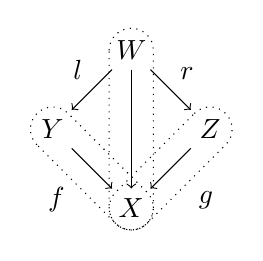
\begin{tikzpicture}[baseline=(Y.base)]
\node(X) at (0, 0) {$X$};
\node(Y) at (-1, 1) {$Y$};
\node(Z) at (1, 1) {$Z$};
\node(W) at (0, 2) {$W$};
\path[->]
(W) edge node[above left]{$l$} (Y)
(W) edge node[above right]{$r$} (Z)
(W) edge (X)
(Y) edge (X)
(Z) edge (X);
\draw[dotted] ([xshift=-5.658pt,yshift=-5.658pt]Y.center) arc (225:45:8pt) -- ([xshift=5.658pt,yshift=5.658pt]X.center) arc (45:-135:8pt) -- cycle;
\draw[dotted] ([xshift=-8pt]W.center) arc (180:0:8pt) -- ([xshift=8pt]X.center) arc (0:-180:8pt) -- cycle;
\draw[dotted] ([xshift=-5.658pt,yshift=5.658pt]Z.center) arc (135:-45:8pt) -- ([xshift=5.658pt,yshift=-5.658pt]X.center) arc (-45:-225:8pt) -- cycle;
\node at (-.95, .1) {$f$};
\node at (.95, .1) {$g$};
\end{tikzpicture}
\qquad\text{which is the same as}\qquad
\begin{tikzpicture}[baseline=($(W)!.5!(X)$)]
\node(X) at (0, 0) {$X$};
\node(XL) at (-1.25, 0) {$X$};
\node(XR) at (1.25, 0) {$X$};
\node(Y) at (-1.25, 1.25) {$Y$};
\node(Z) at (1.25, 1.25) {$Z$};
\node(W) at (0, 1.25) {$W$};
\node at ([yshift=-1pt]$(XL)!.5!(X)$) {$=$};
\node at ([yshift=-1pt]$(X)!.5!(XR)$) {$=$};
\path[->]
(W) edge node[above]{$l$} (Y)
(W) edge node[above]{$r$} (Z)
(W) edge (X)
(Y) edge (XL)
(Z) edge (XR);
\draw[dotted] ([xshift=-8pt]W.center) arc (180:0:8pt) -- ([xshift=8pt]X.center) arc (0:-180:8pt) -- cycle;
\draw[dotted] ([xshift=-8pt]Y.center) arc (180:0:8pt) -- ([xshift=8pt]XL.center) arc (0:-180:8pt) -- cycle;
\draw[dotted] ([xshift=-8pt]Z.center) arc (180:0:8pt) -- ([xshift=8pt]XR.center) arc (0:-180:8pt) -- cycle;
\node at (-1.25, 1.8) {$f$};
\node at (1.25, 1.8) {$g$};
\end{tikzpicture} \]
In a square~|q|, we will refer to the object |Slice.T (Span.M q)|, i.e., the node~|W| in the diagrams above, as the \key{vertex} of~|q|:
\begin{code}
^^^vertex : Square C f g → Object
vertex = Slice.T ∘ Span.M
\end{code}
A product of |f|~and~|g| is alternatively referred to as a \key{pullback} of |f|~and~|g|; that is, it is a square over |f|~and~|g| satisfying
\begin{code}
^^^Pullback C f g : Square C f g → Set _
Pullback C f g = Product (SliceCategory C X) f g
\end{code}
Equivalently, if we define the \key{square category} over |f|~and~|g| as
\begin{code}
^^^SquareCategory C f g : Category
SquareCategory C f g = SpanCategory (SliceCategory C X) f g
\end{code}
then a pullback of |f|~and~|g| is a terminal object in the square category over |f|~and~|g| --- indeed, |Product (SliceCategory C X) f g| is definitionally equal to |Terminal (SquareCategory C f g)|.
This means that, by |terminal-iso|, there is an isomorphism between any two pullbacks |p|~and~|q| of the same slices |f|~and~|g|:
\begin{code}
Iso (SquareCategory C f g) p q
\end{code}
Subsequently, since there is a forgetful functor from |SquareCategory C f g| to~|C| whose object part is |vertex|, and functors preserve isomorphisms, we also have an isomorphism
\begin{flalign}
&\hskip\mathindent |Iso C (vertex p) (vertex q)| &
\label{eq:vertex-iso}
\end{flalign}
which is what we actually use in Sections \ref{sec:ornamental-conversion-isomorphisms}~and~\ref{sec:modularity-isomorphisms}.

Like isomorphisms, we can talk about preservation of pullbacks: any functor |F : Functor C D| maps a square in~|C| into one in~|D|; if the resulting square in~|D| is a pullback whenever the input square in~|C| is, then |F| is said to be \key{pullback-preserving}.
Formally:
\begin{code}
^^^Pullback-preserving F :
  {B : Category.Object C} {f g : Slice C B} (s : Square C f g) →
  Pullback C f g s → Pullback D  (object (SliceMap F) f) (object (SliceMap F) g)
                                 (object (SquareMap F) s)
\end{code}
where
\begin{code}
^^^SliceMap   :  (F : Functor C D) →
                 Functor (SliceCategory C B) (SliceCategory D (object F B))
^^^SquareMap  :  (F : Functor C D) →
                 Functor  (SquareCategory C f g)
                          (SquareCategory D  (object (SliceMap F) f)
                                             (object (SliceMap F) g))
\end{code}
are straightforward liftings of functors on ambient categories to functors on slice and square categories.
Unlike isomorphisms, pullbacks are not preserved by all functors, but the functors |Ind : Functor Ōrn Fam| and |Com : Functor Fam Fun| are pullback-preserving, which we use below.

\subsubsection{Parallel composition as a pullback}

For any |O : Orn e D E| and |P : Orn f D F| where |D : Desc I|, |E : Desc J|, and |F : Desc K|, the following square in |Ōrn| is a pullback:
\begin{equation}
\begin{tikzpicture}[scale=5, baseline=(D.base)]
\node(D) at (1, 0) {|I , D|};
\node(E) at (0, 0) {|J , E|};
\node(F) at (1, .5) {|K , F|};
\node(P) at (0, .5) {|e ⋈ f , ⌊ O ⊗ P ⌋|};
\draw[ultra thick] (.03, .355) -- (.1, .355) -- (.1, .425);
\path[->, font=\small]
(E) edge node[below]{|e , O|} (D)
(F) edge node[right]{|f , P|} (D)
(P) edge node[label on arrow]{|pull , ⌈ O ⊗ P ⌉|} (D)
(P) edge node[left]{\llap{|π₁ , diffOrn-l O P|}} (E)
(P) edge node[above,yshift=.5ex]{|π₂ , diffOrn-r O P|} (F);
\end{tikzpicture}
\label{eq:pc-square}
\end{equation}
We assert that the square is a pullback by marking its vertex with ``\smash{
\begin{tikzpicture}[scale=3.75] \draw[ultra thick] (.03, .355) -- (.1, .355) -- (.1, .425); \end{tikzpicture}}\,''.
The \Agda\ term for the square is
\begin{code}
^^^pc-square O P : Square Ōrn ((J , E) , (e , O)) ((K , F) , (f , P))
pc-square O P =  ((e ⋈ f , ⌊ O ⊗ P ⌋) , (pull , ⌈ O ⊗ P ⌉)) ,
                 ((π₁  , diffOrn-l  O P) , (goal()(0))) ,
                 ((π₂  , diffOrn-r  O P) , (goal()(1)))
\end{code}
where Goal~0 has type |OrnEq (O ⊙ diffOrn-l O P) ⌈ O ⊗ P ⌉| and Goal~1 has type |OrnEq (P ⊙ diffOrn-r O P) ⌈ O ⊗ P ⌉|, both of which can be discharged.
Comparing the commutative diagram~(\ref{eq:pc-square}) and the \Agda\ term |pc-square O P|, it should be obvious how concise the categorical language can be --- the commutative diagram expresses the structure of the \Agda\ term in a clean and visually intuitive way.
Since terms like |pc-square O P| can be reconstructed from commutative diagrams and the categorical definitions, from now on we will present commutative diagrams as representations of the corresponding \Agda\ terms and omit the latter.
A proof sketch of~(\ref{eq:pc-square}) is deferred to \autoref{sec:ornaments-and-horizontal-transformations}.
The pullback property~(\ref{eq:pc-square}) by itself is not too useful in this chapter, though: |Ōrn| is a quite restricted category, so a universal property established in |Ōrn| has limited applicability.
Instead, we are more interested in the following two pullback properties: the image of~(\ref{eq:pc-square}) under |Ind| in |Fam|:
\begin{equation}
\kern5.1pt\begin{tikzpicture}[scale=5, baseline=(D.base)]
\node(D) at (1, 0) {|I , μ D|};
\node(E) at (0, 0) {|J , μ E|};
\node(F) at (1, .5) {|K , μ F|};
\node(P) at (0, .5) {|e ⋈ f , μ ⌊ O ⊗ P ⌋|};
\draw[ultra thick] (.03, .355) -- (.1, .355) -- (.1, .425);
\path[->, font=\small]
(E) edge node[below]{|e , forget O|} (D)
(F) edge node[right]{\rlap{|f , forget P|}} (D)
(P) edge node[label on arrow]{|pull, forget ⌈ O ⊗ P ⌉|} (D)
(P) edge node[left]{\llap{|π₁ , forget (diffOrn-l O P)|}} (E)
(P) edge node[above, yshift=1ex]{|π₂ , forget (diffOrn-r O P)|} (F);
\end{tikzpicture}
\label{eq:Fam-pullback}
\end{equation}
and the image of~(\ref{eq:Fam-pullback}) under |Com| in |Fun|:
\begin{equation}
\begin{tikzpicture}[scale=5, baseline=(D.base)]
\node(D) at (1, 0) {|Σ I (μ D)|};
\node(E) at (0, 0) {|Σ J (μ E)|};
\node(F) at (1, .5) {|Σ K (μ F)|};
\node(P) at (0, .5) {|Σ (e ⋈ f) (μ ⌊ O ⊗ P ⌋)|};
\draw[ultra thick] (.03, .355) -- (.1, .355) -- (.1, .425);
\path[->, font=\small]
(E) edge node[below]{|e * forget O|} (D)
(F) edge node[right]{\rlap{|f * forget P|}} (D)
(P) edge node[label on arrow]{|pull * forget ⌈ O ⊗ P ⌉|} (D)
(P) edge node[left]{\llap{|π₁ * forget (diffOrn-l O P)|}} (E)
(P) edge node[above,yshift=1ex]{|π₂ * forget (diffOrn-r O P)|} (F);
\end{tikzpicture}
\label{eq:Fun-pullback}
\end{equation}
The pullback property of~(\ref{eq:Fam-pullback}) can be directly established.
(Together with the pullback property of~(\ref{eq:pc-square}), this ensures that |Ind| is pullback-preserving --- a functor is pullback-preserving if a specific square and its image under that functor are both pullbacks.)
Then the pullback property of~(\ref{eq:Fun-pullback}) follows from pullback preservation of |Com|.

\section{Consequences}
\label{sec:categorical-consequences}

Characterising parallel composition as a pullback immediately allows us to instantiate standard categorical results, like commutativity |(_ , ⌊ O ⊗ P ⌋) ≅ (_ , ⌊ P ⊗ O ⌋)| and associativity |(_ , ⌊ ⌈ O ⊗ P ⌉ ⊗ Q ⌋) ≅ (_ , ⌊ O ⊗ ⌈ P ⊗ Q ⌉ ⌋)| up to isomorphism in |Ōrn| (which can then be transferred by isomorphism preservation to |Fam|, for example).
Our original motivation, on the other hand, is to implement the ornamental conversion isomorphisms and the modularity isomorphisms, which we carry out below.

\subsection{The ornamental conversion isomorphisms}
\label{sec:ornamental-conversion-isomorphisms}

We restate the ornamental conversion isomorphisms as follows: for any ornament |O : Orn e D E| where |D : Desc I| and |E : Desc J|, we have
\begin{code}
μ E j ≅ (Σ'(x ∶ μ D (e j))) OptP O (ok j) x
\end{code}
for all |j : J|.
Since the optimised predicates |OptP O| are defined by parallel composition of |O|~and the singleton ornamentation |S = singletonOD D|, the isomorphism expands to
\begin{flalign}
&\hskip\mathindent |μ E j ≅ (Σ'(x ∶ μ D (e j))) μ ⌊ O ⊗ ⌈ S ⌉ ⌋ (ok j , ok (e j , x))| &
\label{eq:rep-iso}
\end{flalign}
How do we derive this from the pullback properties for parallel composition?
It turns out that the pullback property~(\ref{eq:Fun-pullback}) in |Fun| can help.

\begin{itemize}

\item Set-theoretically, the vertex of a pullback of two functions |f : A → C| and |g : B → C| is isomorphic to |(Σ'(p ∶ A × B)) f (proj₁ p) ≡ g (proj₂ p)|; the more information |f|~and~|g| carries into~|C|, the stronger the equality constraint.
An extreme case is when |C|~is just~|B| and |g|~is the identity (which retains all information): the equality constraint reduces to |f (outl p) ≡ outr p|, so the second component of~|p| is completely determined by the first component, and thus the vertex is isomorphic to just~|A|.
The same situation happens for the following pullback square:
\begin{equation}
\begin{tikzpicture}[scale=5,baseline=(D.base)]
\node(D) at (1.25, 0) {|Σ I (μ D)|};
\node(E) at (0, 0) {|Σ J (μ E)|};
\node(F) at (1.25, .5) {|Σ (Σ I (μ D)) (μ ⌊ S ⌋)|};
\node(P) at (0, .5) {|Σ J (μ E)|};
\draw[ultra thick] (.04, .355) -- (.11, .355) -- (.11, .425);
\path[->, font=\small]
(E) edge node[below,xshift=-1.2pt]{|e * forget O|} (D)
(F) edge node[right]{\rlap{|proj₁ * forget ⌈ S ⌉|}} (D)
(P) edge node[label on arrow]{|e * forget O|} (D)
(P) edge node[left]{|id|} (E)
(P) edge node[above,yshift=1ex]{|(e * forget O) ▵ (singleton ∘ forget O ∘ proj₂)|} (F);
\end{tikzpicture}
\label{eq:E-square}
\end{equation}
Since singleton ornamentation does not add information to a datatype, the vertical slice on the right-hand side
\begin{code}
s = (Σ (Σ I (μ D)) (μ ⌊ S ⌋)) , (proj₁ * forget ⌈ S ⌉)
\end{code}
retains all information like an identity function, and thus behaves like a ``multiplicative unit'' (viewing pullbacks as products of slices): any (compatible) slice~|s'| alone gives rise to a product of |s|~and~|s'|.
In particular, we can use the bottom-left type |Σ J (μ E)| as the vertex of the pullback.
This pullback square is over the same slices as the pullback square~(\ref{eq:Fun-pullback}) with |P|~substituted by~|⌈ S ⌉|,
so by~(\ref{eq:vertex-iso}) we obtain an isomorphism
\begin{flalign}
&\hskip\mathindent |Σ J (μ E) ≅ Σ (e ⋈ proj₁) (μ ⌊ O ⊗ ⌈ S ⌉ ⌋)| &
\label{eq:rep-iso-raw}
\end{flalign}

\item To get from~(\ref{eq:rep-iso-raw}) to~(\ref{eq:rep-iso}), we need to look more closely into the construction of~(\ref{eq:rep-iso-raw}).
The right-to-left direction of~(\ref{eq:rep-iso-raw}) is obtained by applying the universal property of~(\ref{eq:E-square}) to the square~(\ref{eq:Fun-pullback}) (with |P|~substituted by~|⌈ S ⌉|), so it is the unique mediating morphism~|m| that makes the following diagram commute:
\begin{center}
\begin{tikzpicture}[xscale=3, yscale=3.5, baseline=(E'.base)]
\node(E) at (0, 0) {|Σ J (μ E)|};
\node(E') at (-1, .5) {|Σ J (μ E)|};
\node(S) at (1, .5) {|Σ (Σ I (μ D)) (μ ⌊ S ⌋)|};
\node(P) at (0, 1) {|Σ (e ⋈ proj₁) (μ ⌊ O ⊗ ⌈ S ⌉ ⌋)|};
\path[->, font=\small]
(E) edge node[below left]{|id|} (E')
(E) edge node[below right, align=left]{|(e * forget O) ▵|\\|(singleton ∘ forget O ∘ proj₂)|} (S)
(P) edge node[above left,yshift=-4pt]{|π₁ * forget (diffOrn-l O P)|} (E')
(P) edge node[above right,yshift=-4pt]{|π₂ * forget (diffOrn-r O P)|} (S)
(P) edge[dashed] node[left]{|m|} (E);
\end{tikzpicture}
\end{center}
From the left commuting triangle, we see that, extensionally, the morphism~|m| is just |π₁ * forget (diffOrn-l O P)|.

\item The above leads us to the following general lemma:
if there is an isomorphism
\begin{code}
Σ K X ≅ Σ L Y
\end{code}
whose right-to-left direction is extensionally equal to some |f * g|, then we have
\begin{code}
X k ≅ (Σ'(l ∶ f ⁻¹ k)) Y (und l)
\end{code}
for all |k : K|.
For a justification: fixing |k : K|, an element of the form |(k , x) : Σ K X| must correspond, under the given isomorphism, to some element |(l , y) : Σ L Y| such that |f l ≡ k|, so the set |X k| corresponds to exactly the sum of the sets |Y l| such that |f l ≡ k|.

\item Specialising the lemma above for~(\ref{eq:rep-iso-raw}), we get
\begin{flalign}
&\hskip\mathindent |μ E j ≅ (Σ'(jix ∶ π₁ ⁻¹ j)) μ ⌊ O ⊗ ⌈ S ⌉ ⌋ (und jix)| &
\label{eq:rep-iso-almost}
\end{flalign}
for all |j : J|.
Finally, observe that a canonical element of type |π₁ ⁻¹ j| must be of the form |ok (ok j , ok (e j , x))| for some |x : μ D (e j)|, so we perform a change of variables for the summation, turning the right-hand side of~(\ref{eq:rep-iso-almost}) into
\begin{code}
(Σ'(x ∶ μ D (e j))) μ ⌊ O ⊗ ⌈ S ⌉ ⌋ (ok j , ok (e j , x))
\end{code}
and arriving at~(\ref{eq:rep-iso}).

\end{itemize}

\subsection{The modularity isomorphisms}
\label{sec:modularity-isomorphisms}

The other important family of isomorphisms we should construct from the pullback properties of parallel composition is the modularity isomorphisms, which is restated as follows:
Suppose that there are descriptions |D : Desc I|, |E : Desc J| and |F : Desc K|, and ornaments |O : Orn e D E|, and |P : Orn f D F|.
Then we have
\begin{code}
OptP ⌈ O ⊗ P ⌉ (ok (j , k)) x ≅ OptP O j x × OptP P k x
\end{code}
for all |i : I|, |j : e ⁻¹ i|, |k : f ⁻¹ i|, and |x : μ D i|.
The isomorphism expands to
\begin{flalign}
&\hskip\mathindent |μ ⌊ ⌈ O ⊗ P ⌉ ⊗ ⌈ S ⌉ ⌋ (ok (j , k) , ok (i , x))| & \nonumber \\
&\hskip\mathindent \quad |≅ μ ⌊ O  ⊗ ⌈ S ⌉ ⌋ (j , ok (i , x)) × μ ⌊ P  ⊗ ⌈ S ⌉ ⌋ (k ,  ok (i , x))|
\label{eq:modularity}
\end{flalign}
where again |S = singletonOD D|.
A quick observation is that they are componentwise isomorphisms between the two families of sets
\savecolumns
\begin{code}
M  =  μ ⌊ ⌈ O ⊗ P ⌉ ⊗ ⌈ S ⌉ ⌋
\end{code}
and
\restorecolumns
\begin{code}
N  =  λ case  (ok (j , k), ok (i , x)) mapsto
                μ ⌊ O  ⊗ ⌈ S ⌉ ⌋ (j ,  ok (i , x)) × μ ⌊ P  ⊗ ⌈ S ⌉ ⌋ (k ,  ok (i , x)) endcase
\end{code}
both indexed by |pull ⋈ proj₁| where |pull| has type |e ⋈ f → I| and |proj₁| has type |Σ I X → I|.
This is just an isomorphism in |Fam| between |(pull ⋈ proj₁ , M)| and |(pull ⋈ proj₁ , N)| whose index part (i.e., the isomorphism obtained under the functor |FamF|) is identity.
Thus we seek to prove that both |(pull ⋈ proj₁ , M)| and |(pull ⋈ proj₁ , N)| are vertices of pullbacks of the same slices.

\begin{itemize}

\item We look at |(pull ⋈ proj₁ , N)| first.
For fixed |i|, |j|, |k|, and~|x|, the set
\begin{code}
N (ok (j , k) , ok (i , x))
\end{code}
along with the cartesian projections is a product, which trivially extends to a pullback since there is a forgetful function from each of the two component sets to the \emph{singleton} set |μ ⌊ S ⌋ (i , x)|, as shown in the following diagram:
\[ \begin{tikzpicture}[scale=5, baseline=(D.base)]
\node(D) at (1.25, 0) {|μ ⌊ S ⌋ (i , x)|};
\node(E) at (0, 0) {|μ ⌊ O  ⊗ ⌈ S ⌉ ⌋ (j , ok (i , x))|};
\node(F) at (1.25, .5) {|μ ⌊ P  ⊗ ⌈ S ⌉ ⌋ (k , ok (i , x))|};
\node(P) at (0, .5) {|N (ok (j , k) , ok (i , x))|};
\draw[ultra thick] (.04, .355) -- (.11, .355) -- (.11, .425);
\path[->, font=\small]
(E) edge node[below,yshift=-1ex]{|forget (diffOrn-r O ⌈ S ⌉)|} (D)
(F) edge node[label on arrow]{|forget (diffOrn-r P ⌈ S ⌉)|} (D)
(P) edge node[left]{|proj₁|} (E)
(P) edge node[above]{|proj₂|} (F);
\end{tikzpicture} \]
Note that this pullback square is possible because of the common~|x| in the indices of the two component sets --- otherwise they cannot project to the same singleton set.
Collecting all such pullback squares together, we get the following pullback square in |Fam|:
\begin{equation}\kern41pt
\begin{tikzpicture}[scale=5,baseline=(D.base)]
\node(D) at (1.25, 0) {|Σ I (μ D) , μ ⌊ S ⌋|};
\node(E) at (0, 0) {|e ⋈ proj₁ , μ ⌊ O  ⊗ ⌈ S ⌉ ⌋|};
\node(F) at (1.25, .5) {|f ⋈ proj₁ , μ ⌊ P  ⊗ ⌈ S ⌉ ⌋|};
\node(P) at (0, .5) {|pull ⋈ proj₁ , N|};
\draw[ultra thick] (.04, .355) -- (.11, .355) -- (.11, .425);
\path[->, font=\small]
(E) edge node[below,yshift=-1ex]{|π₂ , forget (diffOrn-r O ⌈ S ⌉)|} (D)
(F) edge node[label on arrow]{|π₂ , forget (diffOrn-r P ⌈ S ⌉)|} (D)
(P) edge node[left]{|_ , proj₁|} (E)
(P) edge node[above]{|_ , proj₂|} (F);
\end{tikzpicture}
\label{eq:N-pullback}
\end{equation}

\item Next we prove that |(pull ⋈ proj₁ , M)| is also the vertex of a pullback of the same slices as~(\ref{eq:N-pullback}).
This second pullback arises as a consequence of the following lemma (illustrated in the diagram below):
In any category, consider the objects $X$, $Y$, their product $X \Leftarrow X \boxtimes Y \Rightarrow Y$, and products of each of the three objects $X$, $Y$, and $X \boxtimes Y$ with an object~$Z$.
(All the projections are shown as solid arrows in the diagram.)
Then $(X \boxtimes Y) \boxtimes Z$ is the vertex of a pullback of the two projections $X \boxtimes Z \Rightarrow Z$ and $Y \boxtimes Z \Rightarrow Z$.
\[ \begin{tikzpicture}[scale=4, baseline=(Z.base)]
\node(X) at (-1, 1) {$X$};
\node(Y) at (1, 1) {$Y$};
\node(Z) at (0, 0) {$Z$};
\node(XY) at (0, 1) {$X \boxtimes Y$};
\node(XZ) at ({0.5*-sin(45)}, {0.5*cos(45)}) {$X \boxtimes Z$};
\node(YZ) at ({0.5*sin(45)}, {0.5*cos(45)}) {$Y \boxtimes Z$};
\node(XYZ) at (0, {0.5*2*cos(45)}) {$(X \boxtimes Y) \boxtimes Z$};
\path[->]
(XY) edge (X)
(XY) edge (Y)
(XZ) edge (X)
(XZ) edge (Z)
(YZ) edge (Y)
(YZ) edge (Z)
(XYZ) edge (XY)
(XYZ) edge (Z)
(XYZ) edge[dash pattern=on 4pt off 1pt on 2pt off 1pt] (XZ)
(XYZ) edge[dash pattern=on 4pt off 1pt on 2pt off 1pt] (YZ);
\draw[ultra thick] ({-(1-0.7)*0.5*2*cos(45)/2+0.04}, {0.5*2*cos(45)-(1-0.7)*0.5*2*cos(45)/2-0.04}) --
                   (0, {0.7*0.5*2*cos(45)}) --
                   ({ (1-0.7)*0.5*2*cos(45)/2-0.04}, {0.5*2*cos(45)-(1-0.7)*0.5*2*cos(45)/2-0.04});
\end{tikzpicture} \]
We again intend to view a pullback as a product of slices, and instantiate the lemma in |SliceCategory Fam (I , μ D)|, substituting all the objects by slices consisting of relevant ornamental forgetful functions in~(\ref{eq:modularity}).
The substitutions are as follows:
\[ \begin{array}{rcl}
X                            & \mapsto & |_ , (_ , forget O)| \\
Y                            & \mapsto & |_ , (_ , forget P)| \\
X \boxtimes Y                & \mapsto & |_ , (_ , forget ⌈ O ⊗ P ⌉)| \\
Z                            & \mapsto & |_ , (_ , forget ⌈ S ⌉)| \\
X \boxtimes Z                & \mapsto & |_ , (_ , forget ⌈ O ⊗ ⌈ S ⌉ ⌉)| \\
Y \boxtimes Z                & \mapsto & |_ , (_ , forget ⌈ P ⊗ ⌈ S ⌉ ⌉)| \\
(X \boxtimes Y) \boxtimes Z  & \mapsto & |_ , (_ , forget ⌈ ⌈ O ⊗ P ⌉ ⊗ ⌈ S ⌉ ⌉)|
\end{array} \]
where $X \boxtimes Y$, $X \boxtimes Z$, $Y \boxtimes Z$, and $(X \boxtimes Y) \boxtimes Z$ indeed give rise to products in |SliceCategory Fam (I , μ D)|, i.e., pullbacks in |Fam|, by instantiating~(\ref{eq:Fam-pullback}).
What we get out of this instantiation of the lemma is a pullback in |SliceCategory Fam (I , μ D)| rather than |Fam|.
This is easy to fix, since there is a forgetful functor from any |SliceCategory C B| to~|C|:
\begin{code}
^^^SliceF : Functor (SliceCategory C B) C
SliceF = record  case  object    = Slice.T
                 sep   morphism  = SliceMorphism.m
                 sep   proofs-of-laws endcase
\end{code}
which is pullback-preserving.
We thus get a pullback in |Fam| of the same slices as~(\ref{eq:N-pullback}) whose vertex is |(pull ⋈ proj₁ , M)|.

\end{itemize}

Having the two pullbacks, by~(\ref{eq:vertex-iso}) we get an isomorphism in |Fam| between |(pull ⋈ proj₁ , M)| and |(pull ⋈ proj₁ , N)|, whose index part can be shown to be identity, so there are componentwise isomorphisms between |M|~and~|N| in |Fun|, arriving at~(\ref{eq:modularity}).

\section{Discussion}
\label{sec:categorical-discussion}

The categorical organisation of the ornament--refinement framework effectively summarises various constructions in the framework under the succinct categorical language.
For example, the functor |Ind| from |Ōrn| to |Fam| is itself a summary of the following:
\begin{itemize}
\item the least fixed-point operation on descriptions (the object part of the functor),
\item the ornamental forgetful functions (the morphism part of the functor),
\item the equivalence on ornaments, which implies extensional equality on ornamental forgetful functions (since functors respect equivalence),
\item the identity ornaments, whose forgetful functions are extensionally equal to identity functions (since functors preserve identity),
\item sequential composition of ornaments, and the fact that the forgetful function for any sequentially composed ornament |O ⊙ P| is extensionally equal to the composition of the forgetful functions for |O|~and~|P| (since functors preserve composition).
\end{itemize}
Most importantly, a categorical pullback structure emerges from the framework, which gives a macroscopic meaning to the microscopic type-theoretical definition of parallel composition (thus ensuring that the definition is not an arbitrary one), and enables constructions of the ornamental conversion isomorphisms and the modularity isomorphisms on a more abstract level.
Compared to the constructions of the isomorphisms using datatype-generic induction in previous work~\citep{Ko-pcOrn}, the constructions presented in this chapter offer more insights and are easier to understand: after establishing the pullback properties of parallel composition, at the root of the ornamental conversion isomorphisms is the intuition that singleton ornamentation does not add information, and the modularity isomorphisms stem from the fact that the \emph{pointwise} conjunction of optimised predicates trivially extends to a pullback.
Also, the categorical constructions are impervious to change of representation of the universes of descriptions and ornaments; modification to the universes only affects constructions logically prior to the pullback property~(\ref{eq:Fam-pullback}).
This statement is empirically verified --- the representation of the universes really had to be changed once after carrying out the categorical constructions, but the consequences of this change of representation were limited.

\citet{Dagand-categorical-ornaments} provided a purely categorical treatment of ornaments using fibred category theory~\citep{Jacobs-categorical-logic-and-type-theory}, which is quite independent of the development in this chapter, though.
They established correspondences between descriptions and ``polynomial functors''~\citep{Gambino-polynomial-functors} and between ornaments and ``cartesian morphisms'', and sketched how several operations on ornaments correspond to certain categorical notions (including pullbacks), all of which are ultimately based on the abstract notion of locally cartesian closed categories.
Methodologically, there is a notable difference between their work and the categorical development in this dissertation: \citeauthor{Dagand-categorical-ornaments} distinguish ``software'' (e.g., descriptions and ornaments) and ``mathematics'' (e.g., polynomial functors and cartesian morphisms) and then make a connection between them, so they can use mathematical notions as inspiration for software constructs.
In the light of the propositions-as-types principle, though, a further step should be taken: rather than merely making a connection between software artifacts that have the necessary level of detail and mathematical objects that possess desired abstract properties, we should design the software artifacts such that they satisfy the abstract properties themselves, all expressed in one uniform language, so the detail of the artifacts can be effectively managed by reasoning in terms of the abstract properties.
In this spirit, category theory is regarded in this dissertation as merely providing an additional set of abstractions formulated within type theory, as opposed to being an independent formalism.
(As a consequence, the reasoning is still essentially type-theoretical, rather than insisting on purely categorical arguments.)
Ornaments are complex, but the complexity is necessary (as justified in \autoref{sec:ornament-refinement-discussion}) and hence can only be somehow managed rather than being neglected by turning attention to similar mathematical objects.
Fortunately, ornaments themselves exhibit useful categorical structure that can be expressed type-theoretically, so we are able to tame the complexity of ornaments by reasoning abstractly in terms of this categorical structure without switching to a fundamentally different formalism.

The results of this chapter are completely formalised in \Agda.
The setoid approach to managing morphism equivalence works reasonably well, being able to express extensional equality (e.g., in |Fun| and |Fam|), proof irrelevance (e.g., in |SpanCategory| and |SliceCategory|), and layered definitions of equality (e.g., morphism equivalence in |SquareCategory| is ultimately defined in terms of morphism equivalence in the ambient category).
However, the approach works only because the formalised theory is still simple enough: for example, isomorphisms of categories in general cannot be defined sensibly, since that requires us to turn sets of objects into setoids as well, and then the setoids of morphisms have to be indexed by setoids and proved to respect equalities of the latter, which quickly becomes unmanageable.
Our modelling of categories is able to evade this problem because both of the isomorphisms of categories in this dissertation (one is between |Ōrn| and |FRef|, and the other will appear in \autoref{sec:ornaments-and-horizontal-transformations}) use identities as their object parts.
As for formalisation of proofs, while the purely categorical lemmas can be encoded by equational reasoning combinators with a reasonable amount of effort, formalisation in general is rather difficult due to \Agda's intensionality and lack of a tactic language for constructing proofs efficiently, which together result in the need of manually constructing proof terms that require complicated handling of equalities.
Also, not all the reasoning presented can be faithfully encoded: For the last two steps of the argument in \autoref{sec:ornamental-conversion-isomorphisms}, it is possible to formalise the lemma and the change of variables individually and chain them together, but the resulting isomorphisms would have a very complicated definition containing plenty of suspended |subst|s.
If these isomorphisms are used to construct the refinement family in the morphism part of |RSem|, it would be terribly difficult to prove that the morphism part of |RSem| preserves equivalence.
The actual formalisation circumvents the problem by fusing the lemma and the change of variables into one step to get a clean \Agda\ definition such that |RSem| preserves equivalence automatically.
While this kind of change of arguments for formalisation seems to be the norm (see, e.g., \citet[Section~4.5]{Avigad-prime-number-theorem}), it could occur more frequently in dependently typed programming due to the requirement that the constructed terms had better be ``pretty'' if they are to be referred to in later types, so even a powerful tactic language probably would not help much, since it is hard to control the form of proofs constructed by tactics.
More experience in tackling this kind of proof-relevant formalisation is needed.
